\chapter{Introduction}
\thispagestyle{empty}
%\epigraph{
%Our greatest glory is not in never falling, 
%but in rising every time we fall.
%}{Confucius}%

\begin{itemize}
        \item Paragraphe qui décrit le paradigme dans lequel la recherche se conduit. 
                Donc matière noire, questions sur sa nature, rôle des 
                lentilles gravitationnelles pour révéler cette masse par la distortion
        \item Mentionner la motivation générale de notre recherche
\end{itemize}

% Possibly rework this to get a more complete picture
La recherche présentée dans ce mémoire approche le problème de cartographier la 
masse gravitationnelle de galaxies-lentilles de façon agnostique. C'est-à-dire que 
l'on ne suppose pas de modèle analytique simple pour résoudre le problème 
de reconstruction non-linéaire et mal posé. Plutôt, cette recherche exploite 
le cadre des machines à inférence récurrentielles (RIM) pour encoder des biais 
inductifs dans un réseaux de neurones qui vont rendre l'inférence de 
paramètres dans un espace à très haute dimension efficace et précise.

Avant de décrire ce travail, je vais introduire les concepts 
et les motivations nécessairent pour contextualiser ma recherche.
En premier lieu, je vais décrire le concept de lentille 
gravitationnelle à la section \ref{sec:lentilles gravitationnelles}. Ensuite, 
je vais décrire quelque concepts lié à l'extraction de profiles de masses 
provenant de large simulation magnétohydrodynamiques à la section 
\ref{sec:simulation magnetohydrodynamique}. 
Cette section sera suivit d'une introduction rapide à quelques concepts liés 
à l'apprentissage machine utiles pour ma recherche
à la section \ref{sec:apprentissage machine}. 
Je vais décrire le formalisme bayesien pour les problème inverse 
qui sous-tend ma recherche à la section \ref{sec:formalisme probleme inverse}.
Finalement, je vais décrire le 
le contexte historique et scientifique qui motive ma recherche 
à la section \ref{sec:contexte}.
%cadre plus large des motivations scientifiques 
%dans lequel cette recherche se situe à la section \ref{sec:motivations}.
%\citep{Morningstar2019}

\section{Lentilles gravitationnelles}\label{sec:lentilles gravitationnelles}

% Plan pour cette section: Dériver eq de la lentille et alpha
% Intro général: deflection de la lumière
%% Approcha a l'intro -> contexte historique à notre pensée sur la déflection de la lumière
%%% Réfraction 
%%%% Ptolémé (Optic, Grèce Antique)
%%%% Ibn Sahl (c. 940 - 1000)
%%%% Snell (1621)-Descartes(1637)
%%%% Principe de Fermat pour expliquer ce phénomène (lettre en 1657, mémoire en 1662)
%%%% Euler (1744) - Lagrange (1760) -> Principe de moindre action et sa solution
%%%% Équations de Maxwell (1861)

%%% Déflection de la lumière par la gravité
%%%% Soldner, J. G. v. (1801–1804). "On the deflection of a light ray from its rectilinear motion, by the attraction of a celestial body at which it nearly passes by". Berliner Astronomisches Jahrbuch: 161–172.
%%%% Einstein 1911
%%%% Einstein 1915 (GR)
%%%% Eddington takes photograph of eclipse 1919
%%%% 1936 letter from Einstein at the request of 
%%%% Fritz Zwicky is first to postulate grav lensing idea in 1937i Zwicky, F. (1937) Nebulae as gravitational lenses. Physical Review, 51 (4). p. 290. ISSN 0031-899X
%%%% 1964 Refsdal (H0 and possibility to measure mass)
%%%%%% (Shapiro time delay (1964))
%%%% Fisrt gravitational lens discovered 1979 (double imaged quasar) https://www.nature.com/articles/279381a0
%%%% Then explosions of studies durings the 2000s on how to model things.

%%% Dark matter 
%%%% Zwicky 1933
%%%% Lambda CDM?
%%%% 

% Copied from https://royalsocietypublishing.org/doi/10.1098/rsta.2009.0209
%Henry Cavendish in 1784 is credited with the first (unpublished) calculation of the deflection angle 
%δ of a corpuscular light ray following a hyperbolic trajectory and the origin of the 
%(Newtonian) equation δ=2GM/Rc2. Subsequently, von Soldner (1804) published a similar calculation 
%deriving a deflection of 0.84 arcsec for stars viewed close to the limb of the Sun.

%Le principe de Fermat énonce que la trajectoire de la lumière, ou d'un 
%photon, doit suivre une trajectoire qui extrémise la durée de la trajectoire. 
%Ce principe mathématique, qui est un exemple du principe plus général de moindre action 
%développé par Lagrange en 1756, permet de décrire la trajectoire de la lumière 
%par l'entremise d'un simple indice $n$ (indice de réfraction) dans 
%lequel se cache toute la physique microscopique (ou macroscopique) 
%d'où émerge le phénomène qui nous intéresse. 


%L'expédition organisée par sir Arthur Eddington
%avait pour but d'observer 
%l'éclipse totale du 29 mai 1919 à partir de l'île de Prìncipe 
%dans le golfe de Guinée et de Sobral au nord du Brésil 
%\citep{Eddington1919}. Les photographes de l'éclipses prisent , bien qu'imprécises, 
%ont permis de valider la prédiction d'Einstein faite 
%en 1911 que la position observée d'une étoile serait déplacée de 
%$\delta \theta \approx 1.75'' \frac{R}{R_\odot}$ 
%durant une eclipse \citep{Dyson1920}, soit 2 fois plus 
%que ce qui est prédit par la théorie newtonienne.

% Je dois demander un cpoyright authorisation pour utiliser ces images
%\begin{figure}[H]
        %\centering
        %\begin{subfigure}[b]{0.45\linewidth}
                %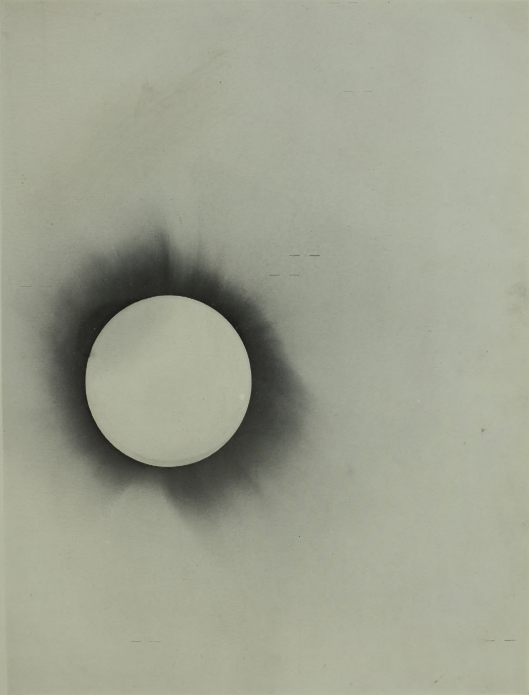
\includegraphics[width=\textwidth]{figures/eddington_photo_royalsociety}
                %\caption{Crédit}
        %\end{subfigure}
        %\hfill
        %\begin{subfigure}[b]{0.45\linewidth}
                %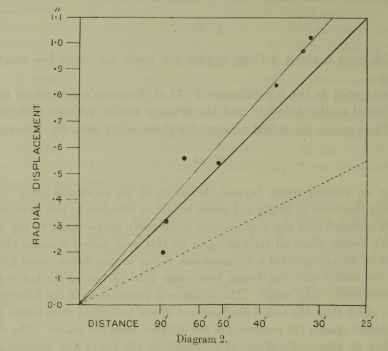
\includegraphics[width=\linewidth]{figures/1919_results_royalsociety}
        %\end{subfigure}
%\end{figure}

L'idée des lentilles gravitationnelles est attribuée a Fritz \citet{Zwicky1937} %(1937) 
qui, suivant les calculs publié par \citet{Einstein1936} l'année précédente, %\citep{Einstein1936},
est le premier à postuler correctement que l'anneau d'Einstein produit par la déflection 
de la lumière d'une source en arrière plan par le champ gravitationnel d'une galaxie 
(appellée nébuleuse extra-galactique à l'époque) 
pourrait être observé. Une idée qu'Einstein lui-même considérait improbable. 
Dans le même article, il articule précisément les idées qui nous motivent encore aujourd'hui 
(presque 100 ans plus tard) à étudier ces objets, 
c'est-à-dire que les lentilles gravitationnelles permettent
\begin{itemize}
        \item d'imager des galaxies trop lointaine pour que l'on puisse les résoudre avec 
                nos téléscopes;
        \item de mesurer directement la masse gravitationnelle de ces galaxies.
\end{itemize}
Pour comprendre ces deux points, 
et dans l'intérêt de rendre ce manuscrit complet, je vais dériver à partir de principes 
premier les équations 
centrales qui nous permettent d'étudier les lentilles gravitationnelles décrites par 
Zwicky.
Des traitements similaires 
peuvent être trouvé dans les manuels de références de \citet{Meneghetti2013} et 
\citet{Carroll2003}.

\subsection{Les angles de déflections}
Un angle de déflection est la déviation angulaire apparente d'un point 
lumineux par rapport à sa position originelle si 
le chemin du photon n'était pas dévié. Pour rendre les dérivations simples, 
on sépare les coordonnées en une partie parallèle à l'axe de visée de l'observateur ($\mathbf{e}_\parallel$) 
et une partie perpendiculaire ($\mathbf{e}_\perp$). L'angle de déflection se calcule entièrement 
dans la partie perpendiculaire. Sans assumer la nature de cette déflection, 
on peut écrire de façon générale
\begin{equation}\label{eq:alpha}
        \boldsymbol{ \alpha} = - \int_{\lambda_A}^{\lambda_B} \ddot{\mathbf{x}} \times \mathbf{e}_{\parallel} d\lambda,
\end{equation}
où $\lambda$ paramétrise la trajectoire du photon, et $\mathbf{x}$ est un vecteur de 
position. Le signe moins nous indique qu'on prend la perspective de l'observateur. 
%Je note que sous cette forme, l'équation est difficile à résoudre puisque 
%$\mathbf{e}_{\parallel}$ dépend généralement de $\lambda$.

Le principe de Fermat stipule que la lumière suit une trajectoires qui extrémise
la durée de son parcours entre deux points. 
C'est un exemple du principe 
plus général de moindre action développé par Lagrange. 
C'est pourquoi le principe de Fermat est formalisé dans le language du calcul 
des variations, où la variation de la durée $T$ s'écrit
\begin{equation}\label{eq:Fermat}
        %\delta T =  \delta \int_{\lambda_A}^{\lambda_B} n(\mathbf{x}(\lambda)) \frac{\lVert d \mathbf{x} \rVert}{d\lambda }  \frac{d\lambda}{c} = 0 
        \delta T =  \delta \int_{A}^{B} n(\mathbf{x}(\ell)) \frac{d\ell}{c}= 0 .
\end{equation}
$n$ est un indice de réfraction et $\ell$ est un élément de longueur sur 
la trajectoire.
Pour déterminer l'indice de réfraction du champ gravitationnel d'une galaxie, 
on utilise le formalisme de la relativité générale. On fait l'approximation 
que le potentiel $\Phi$ de cet galaxie est celui d'un gas parfait, c'est à dire 
qu'il satisfait une équation de Poisson
\begin{equation}\label{eq:Poisson}
       \grad^{2}\Phi = 4\pi G \rho .
\end{equation} 
Dans la limite où ce potentiel est faible $\displaystyle \frac{2\Phi}{c^{2}} \ll 1$, la 
métrique $g_{\mu \nu}$ est décrite par une expansion au premier ordre autour de la 
métrique de Minkowsky $\eta_{\mu\nu}$
\begin{equation}\label{eq:metrique}
        ds^2 = g_{\mu\nu}dx^{\mu}dx^{\nu} \approx \left( 1 + \frac{2\Phi}{c^{2}} \right)c^{2}dt^{2} - \left( 1 - \frac{2\Phi}{c^{2}} \right)d\mathbf{x}^{2}.
\end{equation} 
Puisqu'un photon suit une géodésique de l'espace-temps $ds^{2} = 0$, on peut déterminer 
$n$ en réarrengeant l'équation \eqref{eq:metrique}
\begin{equation}\label{eq:n}
        n = c \left( \frac{\lVert d \mathbf{x} \rVert}{dt}  \right)^{-1} \approx  1 - \frac{2\Phi}{c^{2}}.
\end{equation} 
On peut alors résoudre l'équation \eqref{eq:Fermat} 
en réintroduisant le paramètre de la trajectoire $\lambda$
\begin{equation}\label{eq:ell}
        d\ell = \left\lVert\frac{d  \mathbf{x} }{d\lambda} \right\rVert d\lambda .
\end{equation} 
La trajectoire $\mathbf{x}(\lambda)$ est une solution des équations d'Euler-Lagrange
\begin{equation}\label{eq:EulerLagrange}
        \frac{d }{d \lambda} \frac{\partial \mathcal{L}}{\partial \dot{\mathbf{x}}} - \frac{\partial \mathcal{L}}{\partial \mathbf{x}} = 0 ,
\end{equation} 
où $\mathcal{L} = n(\mathbf{x})  \sqrt{\dot{\mathbf{x}}^{2}}$. On a donc
\begin{equation}\label{eq:EulerLagrange2}
        \frac{d }{d \lambda} n \frac{\dot{\mathbf{x}}}{\lVert \dot{\mathbf{x}} \rVert}- \lVert \dot{\mathbf{x}} \rVert \grad n = 0 ,
\end{equation} 
Puisque le choix du paramètres $\lambda$ est libre, on peut le choisir tel 
que $\lVert \dot{\mathbf{x}} \rVert = 1$ en tout point de la trajectoire. Ainsi,
\begin{equation}\label{eq:EulerLagrange3}
\begin{aligned}
        \frac{d }{d \lambda} n \dot{\mathbf{x}} -  \grad n &= 0 \\
        \implies n \ddot{\mathbf{x}} + (\grad n \cdot \dot{\mathbf{x}}) \dot{\mathbf{x}} - \grad n &= 0
\end{aligned}
\end{equation} 
À ce point de la dérivation, on utilise l'approximation de Born. 
C'est-à-dire qu'on approxime la trajectoire 
du photon comme une ligne droite sur l'axe de visée $\mathbf{e}_{\parallel}$. 
Cette approximation est justfiée 
dans le contexte des lentilles gravitationnelles, 
puisque les angles de déflection sont généralement de 
l'ordre de l'arcseconde ou plus petit. 
Comme, le vecteur $\dot{\mathbf{x}}$ est tangent à la trajectoire du photon, 
on obtient
\begin{equation}\label{eq:sol}
        \ddot{\mathbf{x}} \times \mathbf{e}_{\parallel} = \frac{1}{n} \grad_\perp n = \grad_\perp \log n
        \approx -\frac{2}{c^{2}}\grad_{\perp} \Phi
\end{equation} 
On note que le facteur 2 introduit dans l'équation \eqref{eq:sol} est un 
effet qui vient de la relativité générale. Ce facteur corrige la solution 
que l'on aurait obtenu avec une dérivation newtonienne.

On introduit le paramètre d'impact $\boldsymbol{\xi}$ qui est la distance perpendiculaire entre 
la position d'origine du photon sur le plan de la lentille  
et l'axe de visé (voir la figure \ref{fig:cartoon}). 
Dans le cas où le potentiel est généré par une masse $M$ ponctuelle, ç.-à-d. qu'on 
suppose $\rho = M\delta^{3}(\mathbf{x})$ où $\delta $ est la fonction delta de Dirac, 
alors le potentiel qui satisfait l'équation de Poisson est 
la fonction de Green 
$\displaystyle \Phi = -\frac{GM}{\sqrt{ \boldsymbol{\xi}^{2} + z^{2}}}$, où $z$ est la coordonné 
sur l'axe de visée. On a finalement 
\begin{equation}\label{eq:deflection approx}
        \boldsymbol{ \alpha}(\boldsymbol{ \xi} ) = \frac{2GM}{c^{2}} \boldsymbol{ \xi}  
        \int_{-\infty }^{\infty } \frac{dz}{(\boldsymbol{ \xi} ^{2} + z^{2})^{3/2}} 
        = \frac{4GM}{c^{2}  \boldsymbol{ \xi}^{2} } \boldsymbol{ \xi}
\end{equation} 
Cette solution se généralise naturellement à un profil de masse quelconque en assumant 
qu'il s'exprime comme une somme d'élément de masses $dm = \Sigma d^{2}\boldsymbol{ \xi}'$ 
où $\Sigma = \int \rho dz$ est un densité surfacique de masse. 
L'angle de déflection total mesuré à un point $\boldsymbol{\xi} $ est alors une convolution 
sur tout le plan de la lentille (mince) puisque l'équation \eqref{eq:deflection approx} dépend 
linairement de la masse $M$:
\begin{equation}\label{eq:alpha physique}
        \boldsymbol{ \alpha} (\boldsymbol{ \xi} ) = \frac{4 G}{c^{2}} 
        \int_{\mathbb{R}^{2}} \Sigma (\boldsymbol{ \xi} ')
        \frac{\boldsymbol{ \xi}  - \boldsymbol{ \xi} '}{\lVert \boldsymbol{ \xi}  - \boldsymbol{ \xi} ' \rVert^{2}}d^{2}\boldsymbol{ \xi} '
\end{equation} 

\begin{figure}[H]
        \centering
        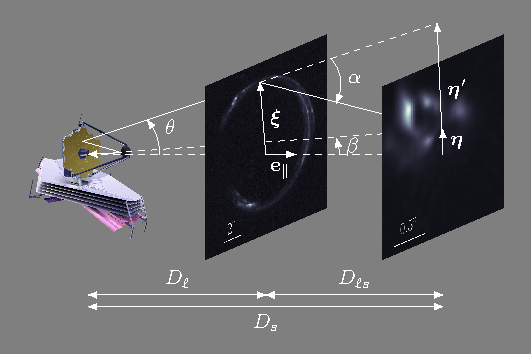
\includegraphics[width=\textwidth]{figures/lensing_cartoon}
        \caption{Schéma d'une lentille gravitationnelle.}
        \label{fig:cartoon}
\end{figure}

\subsection{L'équation de la lentille}

Pour faire une image du plan source, on doit retrouver la position angulaire 
d'un point lumineux à la source $\boldsymbol{ \beta}$ à partir de sa position angulaire
observée $\boldsymbol{ \theta} $ et de nos connaissances sur la déflection $\boldsymbol{ \alpha}$. 
On assume que les distances $D_{\ell}$, $D_s$ et $D_{\ell s}$ sont beaucoup 
plus grandes que les distances perpendiculaires $\boldsymbol{ \xi} $ ou $\boldsymbol{ \eta} $ 
(voir figure \ref{fig:cartoon}). 
Pour les objets qui nous intéresses, les distances parallèles à l'axe de visée sont généralement 
de l'ordre du Gpc, alors que les distances perpendiculaire sont généralement 
de l'ordre du kpc, soit 6 ordres de grandeurs de différences.
Ainsi, on peut faire l'argument géométrique
\begin{equation}\label{eq:lens equation}
       \begin{aligned}
               D_{s} \boldsymbol{ \theta} &= \boldsymbol{ \eta}' \\   
               D_{s} \boldsymbol{ \beta} &= \boldsymbol{ \eta} \\   
               D_{\ell s} \boldsymbol{ \alpha} &= \boldsymbol{ \eta}' - \boldsymbol{ \eta}  \\   
               \implies D_s \boldsymbol{ \beta} &= D_s \boldsymbol{ \theta} - D_{\ell s} \boldsymbol{ \alpha}   
       \end{aligned} 
\end{equation} 
C'est l'équation maîtresse qui nous permet de tracer les rayons lumineux d'une source 
vers un détecteur fictif dans nos simulations.

Dans les équations précédentes, on a assumé qu'une 
longueur physique et l'angle qui sous-tend cette longueur à une certaine distance 
$D$ sont reliés géométriquement dans un espace euclidien (plat). Or, étant donné 
les distances cosmologiques (Gpc) parcouru par les photons avant la capture par nos détecteurs, 
on doit tenir compte du phénomène de l'expansion de l'Univers et en général de sa courbure 
pour déterminer les distances perpendiculaires réelles. C'est pourquoi on utilise plutôt 
le concept de distance du diamètre angulaire (de l'anglais \textit{angular diameter distance}) 
lorsqu'on manipule l'équation de la lentille. On commence par définir cette distance par 
la relation euclidienne entre une longueur $\ell$ et un angle observé $\theta$:
\begin{equation}\label{eq:D}
        D \equiv \frac{\ell}{\theta}
\end{equation} 
On doit maintenant déterminer comment $\ell$ et $\theta$ se comportent en fonction de 
la distance. Pour se faire, on doit faire certaines suppositions par rapport 
à notre Univers. Mon traitement s'inspire des dérivations qu'on peut trouver 
dans les textes de références de \citet{Dodelson2003}, \citet{Carroll2003}, \citet{Rindler2006} et 
\citet{Weinberg2008}.

Il est généralement plaisant de commencer cette dérivation en statuant le postulat de 
Copernic: \textit{il n'existe aucun point de vue privilégié dans l'Univers}. Dans un sens, 
ce postulat nous encourage à se mettre dans la peau d'un être conscient observant le ciel 
à partir d'une autre planète, où même d'une autre galaxie. Cet observateur devrait être en 
mesure de parvenir aux même conclusions que nous sur la structure générale de l'Univers. 
Il est tout à fait raisonnable de protester 
que l'environnement proche de cet observateur soit bien différent 
du notre. Mais, en portant ses observations à grande échelle où les différences locales 
entre différentes galaxies ou systèmes planétaires disparaissent dans une agrégation statistiques, 
alors les conclusions de cet observateur devrait s'accorder avec nos conclusions.

Ceci nous mène à postuler le principe cosmologique: 
\textit{l'Univers est spatiallement homogène et localement isotrope}.
%On notera que ce principe ne dit rien sur les symétries temporelle de l'Univers. 
%Cette concession est forcé par l'observation de l'expansion de l'Univers, formulé 
%sous la loi de Hubble-Lemaître.

%(phot de SDSS)
%metrique FLRW
%assume univers plat (k=0)
%distance comobile -> ell
%redshift
%distance angulaire
\begin{figure}[H]
        \centering
        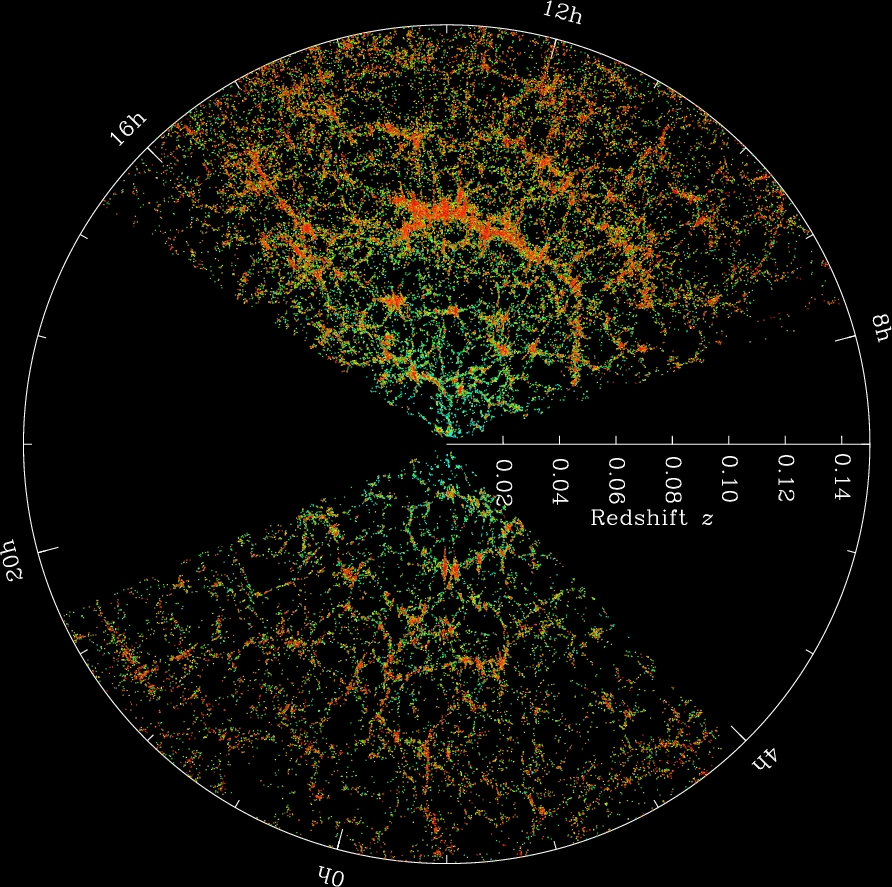
\includegraphics[width=\textwidth]{figures/sdss_universe}
        \caption{Carte des galaxies prise par le Sloan Digital Sky Survey telescope montrant 
        le niveau d'homogénéité et d'isotropie de l'Univers local. Chaque point est 
        coloré par le niveau de densité local.}
        \label{fig:sdss}
\end{figure}


\section{Simulation magnétohydrodynamiques}\label{sec:simulation magnetohydrodynamique}
Les détails de ces simulations tombent en dehors du cadre de cette thèse, 
toutefois on peut noter que plusieurs simulations de haute qualité sont maintenant 
capable de reproduire plusieurs observables de l'Univers d'aujourd'hui ($z=0$). 
Ainsi, on peut utiliser ces simulations pour créer des profils de masses 
autrement inaccessible par des observations qui sont basées uniquement 
sur le champ électromagnétique de l'Univers.

Introduire SPL, main equation.
\begin{itemize}
        \item Devrait être courte, mais établir le ground work pour 
                SPL
        \item Décrire généralement les éléments intéressants d'Illustris, et
                comment en général ce genre de simulations sont pertinentes 
                pour notre travail -> realistic mass models.
\end{itemize}
%\subsection{Description lissée des particules}

%\subsection{Arbres kd}
 
\subsection{Densité de masse projeté avec lissage adaptif}
Introduire les concepts nécessaires pour justifié notre utilisation de 
lissage adaptif pour réduire les erreurs sur les angles de déflections.


\section{Apprentissage machine}\label{sec:apprentissage machine}

\subsection{Réseaux de neuronnes convolutionnels}
Mentionner les travaux de Courville et les avancées récentes.

\subsection{Réseaux de neuronnes récurrents}
Mentionner les résultats importants concernant Turing machines. 
Mentionner les détails d'un GRU convolutifs.

%\subsection{Machine à inférence récurrentielles}


\subsection{Auto-encodeur variationnel}
Inclure ici l'appendice de l'article en plus ou moins de détail.

\subsection{Transfert de l'apprentissage}
Introduction générale.
Inclure ici l'appendice de l'article?

\section{Formalisme des problèmes inverses}\label{sec:formalisme probleme inverse}

%\subsection{Approche bayesienne}

%\subsection{Biais inductifs}

%\subsection{}


\section{Contexte scientifique}\label{sec:contexte}



